\documentclass[border=3pt]{standalone}
% Preâmbulo compartilhado pelos diagramas TikZ da aula 4 de Navegação (Representação de Mapas)
\usepackage[T1]{fontenc}
\usepackage[utf8]{inputenc}
\usepackage{lmodern}
\usepackage{amsmath}
\usepackage{xcolor}
\usepackage{tikz}
\usetikzlibrary{arrows.meta,angles,quotes,decorations.pathmorphing,decorations.pathreplacing,calc,
                positioning,shapes.geometric,shapes.misc,backgrounds,fit,
                math}

% Paleta (mesma dos SVGs originais)
\definecolor{dblue}{HTML}{2A5B8C}
\definecolor{dorange}{HTML}{B3541E}
\definecolor{dgreen}{HTML}{4A7C59}
\definecolor{dred}{HTML}{9C4B4B}
\definecolor{dcream}{HTML}{F4F1EA}
\definecolor{dshade}{HTML}{DDD7C9}

% Função gaussiana (não normalizada por padrão de escala visual)
\pgfmathdeclarefunction{gauss}{3}{%
  \pgfmathparse{1/(#3*sqrt(2*pi))*exp(-((#1-#2)^2)/(2*#3^2))}%
}

% Estilos comuns (prefixo d... para não colidir com chaves internas do pgf)
\tikzset{
  >={Stealth[length=2mm]},
  dguide/.style={gray!55, dashed, line width=0.4pt},
  daxis/.style={gray!60, line width=0.7pt, ->},
  dbody/.style={fill=black!3, draw=black!80, line width=1pt},
  dacc/.style={draw=dblue, line width=1pt},
  dlbl/.style={black!55, font=\small},
  dsub/.style={black!45, font=\footnotesize},
  dstate/.style={circle, draw=black!80, fill=dcream, line width=1pt,
                 minimum size=17mm, font=\large, inner sep=1pt},
  dobs/.style={circle, draw=black!80, fill=dshade, line width=1pt,
               minimum size=14mm, font=\large, inner sep=1pt},
  dbox/.style={rounded corners=2pt, draw=black!80, fill=dcream, line width=1pt,
               align=center, inner sep=6pt},
  dop/.style={circle, draw=black!80, fill=white, line width=1pt,
              minimum size=6mm, inner sep=0pt, font=\small},
  dtrans/.style={->, dblue, line width=1pt},
  dmeas/.style={->, dorange, line width=1pt},
  dcurve/.style={line width=1pt, dblue},
  dcurveb/.style={line width=1.4pt, dorange},
}

\begin{document}
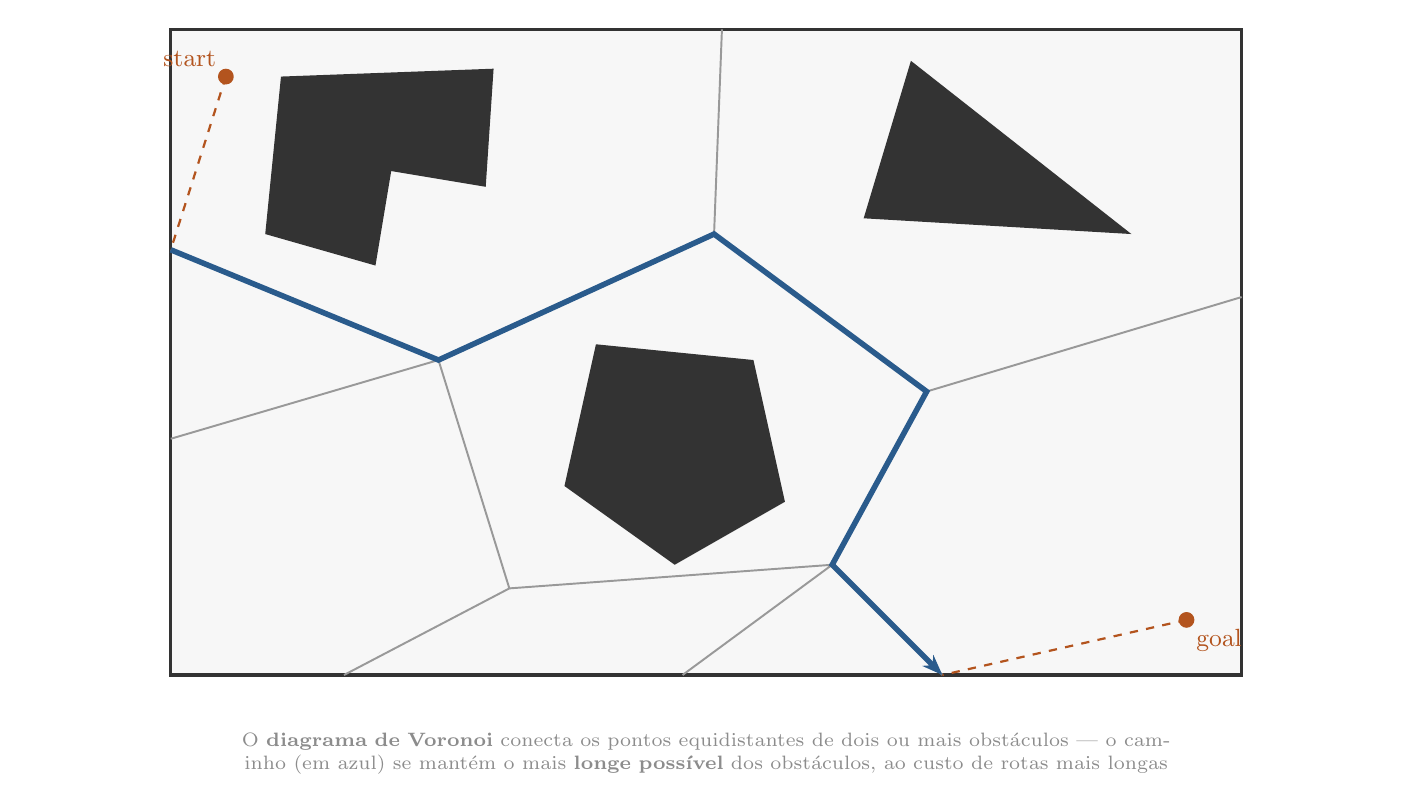
\begin{tikzpicture}[x=1cm,y=1cm]

  \draw[dbody, line width=1.2pt] (0,0) rectangle (13.6,8.2);

  % Obstáculos
  \fill[black!80] (1.4,7.6) -- (1.2,5.6) -- (2.6,5.2) -- (2.8,6.4) -- (4.0,6.2) -- (4.1,7.7) -- cycle;
  \fill[black!80] (9.4,7.8) -- (8.8,5.8) -- (12.2,5.6) -- cycle;
  \fill[black!80] (5.4,4.2) -- (5.0,2.4) -- (6.4,1.4) -- (7.8,2.2) -- (7.4,4.0) -- cycle;

  % Junções do diagrama de Voronoi (equidistantes dos obstáculos/fronteiras)
  \coordinate (j1) at (3.4,4.0);
  \coordinate (j2) at (6.9,5.6);
  \coordinate (j3) at (4.3,1.1);
  \coordinate (j4) at (9.6,3.6);
  \coordinate (j5) at (8.4,1.4);

  \draw[black!40, line width=0.7pt]
    (0,5.4) -- (j1) -- (0,3.0)
    (j1) -- (j2) -- (7.0,8.2)
    (j2) -- (j4) -- (13.6,4.8)
    (j1) -- (j3) -- (2.2,0)
    (j3) -- (j5) -- (6.5,0)
    (j5) -- (j4)
    (j5) -- (9.8,0);

  \coordinate (start) at (0.7,7.6);
  \coordinate (startp) at (0,5.4);
  \coordinate (goal) at (12.9,0.7);
  \coordinate (goalp) at (9.8,0);

  \draw[dorange, dashed, line width=0.8pt] (start) -- (startp);
  \draw[dorange, dashed, line width=0.8pt] (goal) -- (goalp);

  \draw[dblue, line width=2pt, -{Stealth[length=2.6mm]}]
    (startp) -- (j1) -- (j2) -- (j4) -- (j5) -- (goalp);

  \fill[dorange] (start) circle (0.1);
  \node[dorange, font=\small, anchor=south east] at (start) {start};
  \fill[dorange] (goal) circle (0.1);
  \node[dorange, font=\small, anchor=north west] at (goal) {goal};

  \node[dsub, font=\scriptsize, align=center, text width=17cm] at (6.8,-1.0)
     {O \textbf{diagrama de Voronoi} conecta os pontos equidistantes de dois ou mais obstáculos --- o caminho (em azul) se mantém o mais \textbf{longe possível} dos obstáculos, ao custo de rotas mais longas};

\end{tikzpicture}
\end{document}
